%!TEX root=paper.tex

\newpage
\section{The System}
\label{sec:system}

Our vision for the long term is that of an open educational ecosystem in which different creators can share information among their applications in order to maximize the level of personalization that learners percieve. Various reader applications could share information with various vocabulary training applications all mediated by a common API that would track an evolving knowledge model of the learners\cite{Lungu16}.

% by interacting with a core API that provides the basic contextual translations, user knowledge estimation, and recommendations for words to be studied and texts to be read \cite{Lungu16}. 

To show the potential of such an ecosystem we started by implementing ourselves several of the basic components of the ecosystem which together provide the full experience of a {\em personalized language textbook}: 

\begin{description}

  \item [Article Reader] -- consists of a feed subscription mechanism, an article browser that presents the results of crawling the selected feeds that the user is interested in and a web-based interactive text reader which provides seamless in place translations
  
  \item [Vocabulary Trainer] -- which consists of an exercise platform which generates exercises based on a reader's past reading experience

  \item [Translation Service] -- a component responsible with automatically translating words and groups of words from online texts is critical to the system

\end{description}


The components that we present here are implemented using HTML5 and Javascript technologies for the front end and Python and Flask for the backend. For the frontend, we have experienced in the past with writing native applications, however, the interaction with the native elements was too clumsy. Therefore, the user interface elements that we present here are designed as a responsive HTML that can be used on any device. 

Moreover, maintaining multiple systems for multiple platforms is too expensive for an academic environment. The decision turned out to be practical since the users of our system come from multiple platforms.


\subsection{Article Reader}

The Article Reader allows the learners to subscribe to various sources of articles (e.g. websites, blogs) and provides a convenient interaction for reading and translating unknown words. It consists of several components:

\newpage
\subsubsection{Subscription Mechanism}
\ml{make sure that we use source consistently in the text; not feed for example.}
From the user's point of view, the Article reader is organized around sources. When the user indicates that they would like to subscribe to a new source the subscription dialog is displayed. The system categorizes sources by their language and users can select different article sources every language. 

    \begin{figure}[h!]
    \centering
      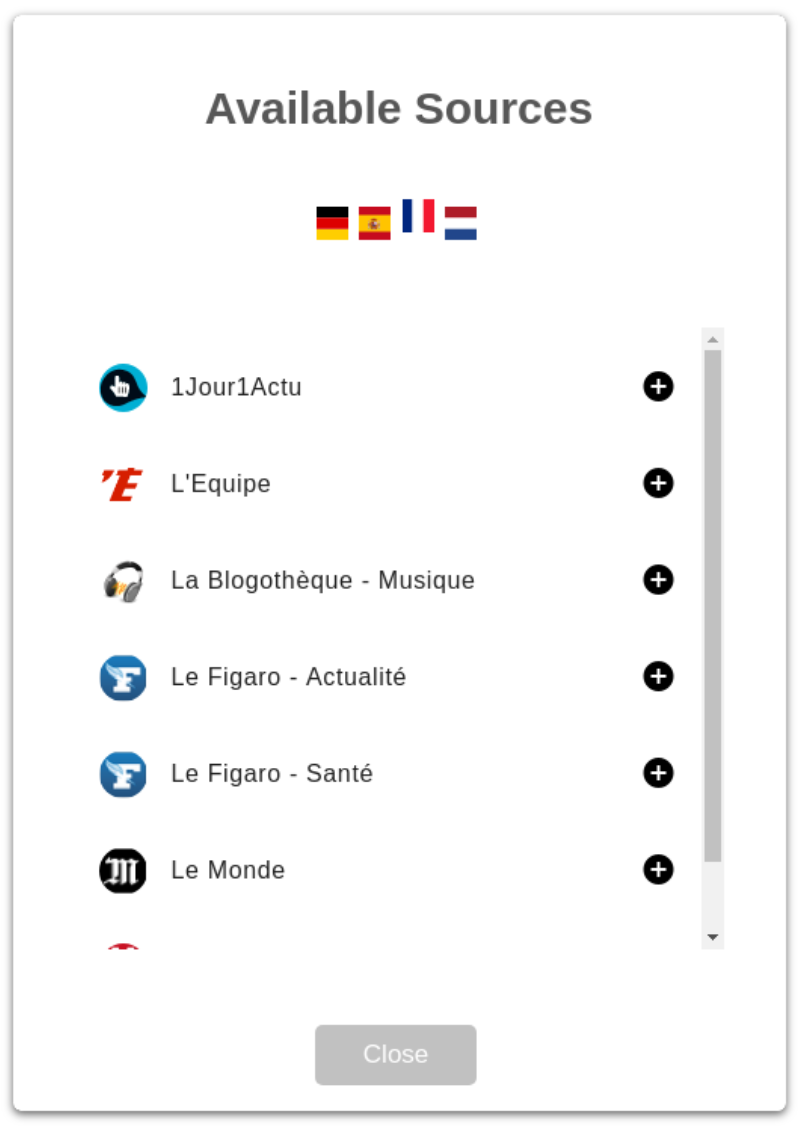
\includegraphics[width=0.4\columnwidth]{figures/available_sources}
      \caption{Different users subscribe to different sources}~\label{fig:system_subscriptions}
    \end{figure}


Figure \ref{fig:system_subscriptions} illustrates multiple sources for the French language, which is being selected at the moment. 
% , as their compact and iconic representation should be universally understood.
At the moment, multiple sources for every language are pre-loaded in the system and if a reader wants to add a new source they have to send an email to the maintainers of the system. 

A multi-lingual learner can subscribe to multiple sources in different languages. 

\subsubsection{Article Browser}

Article listing presents the source, a summary of the article, and an estimated difficulty level of the article.

    \begin{figure}[h!]
    \centering
      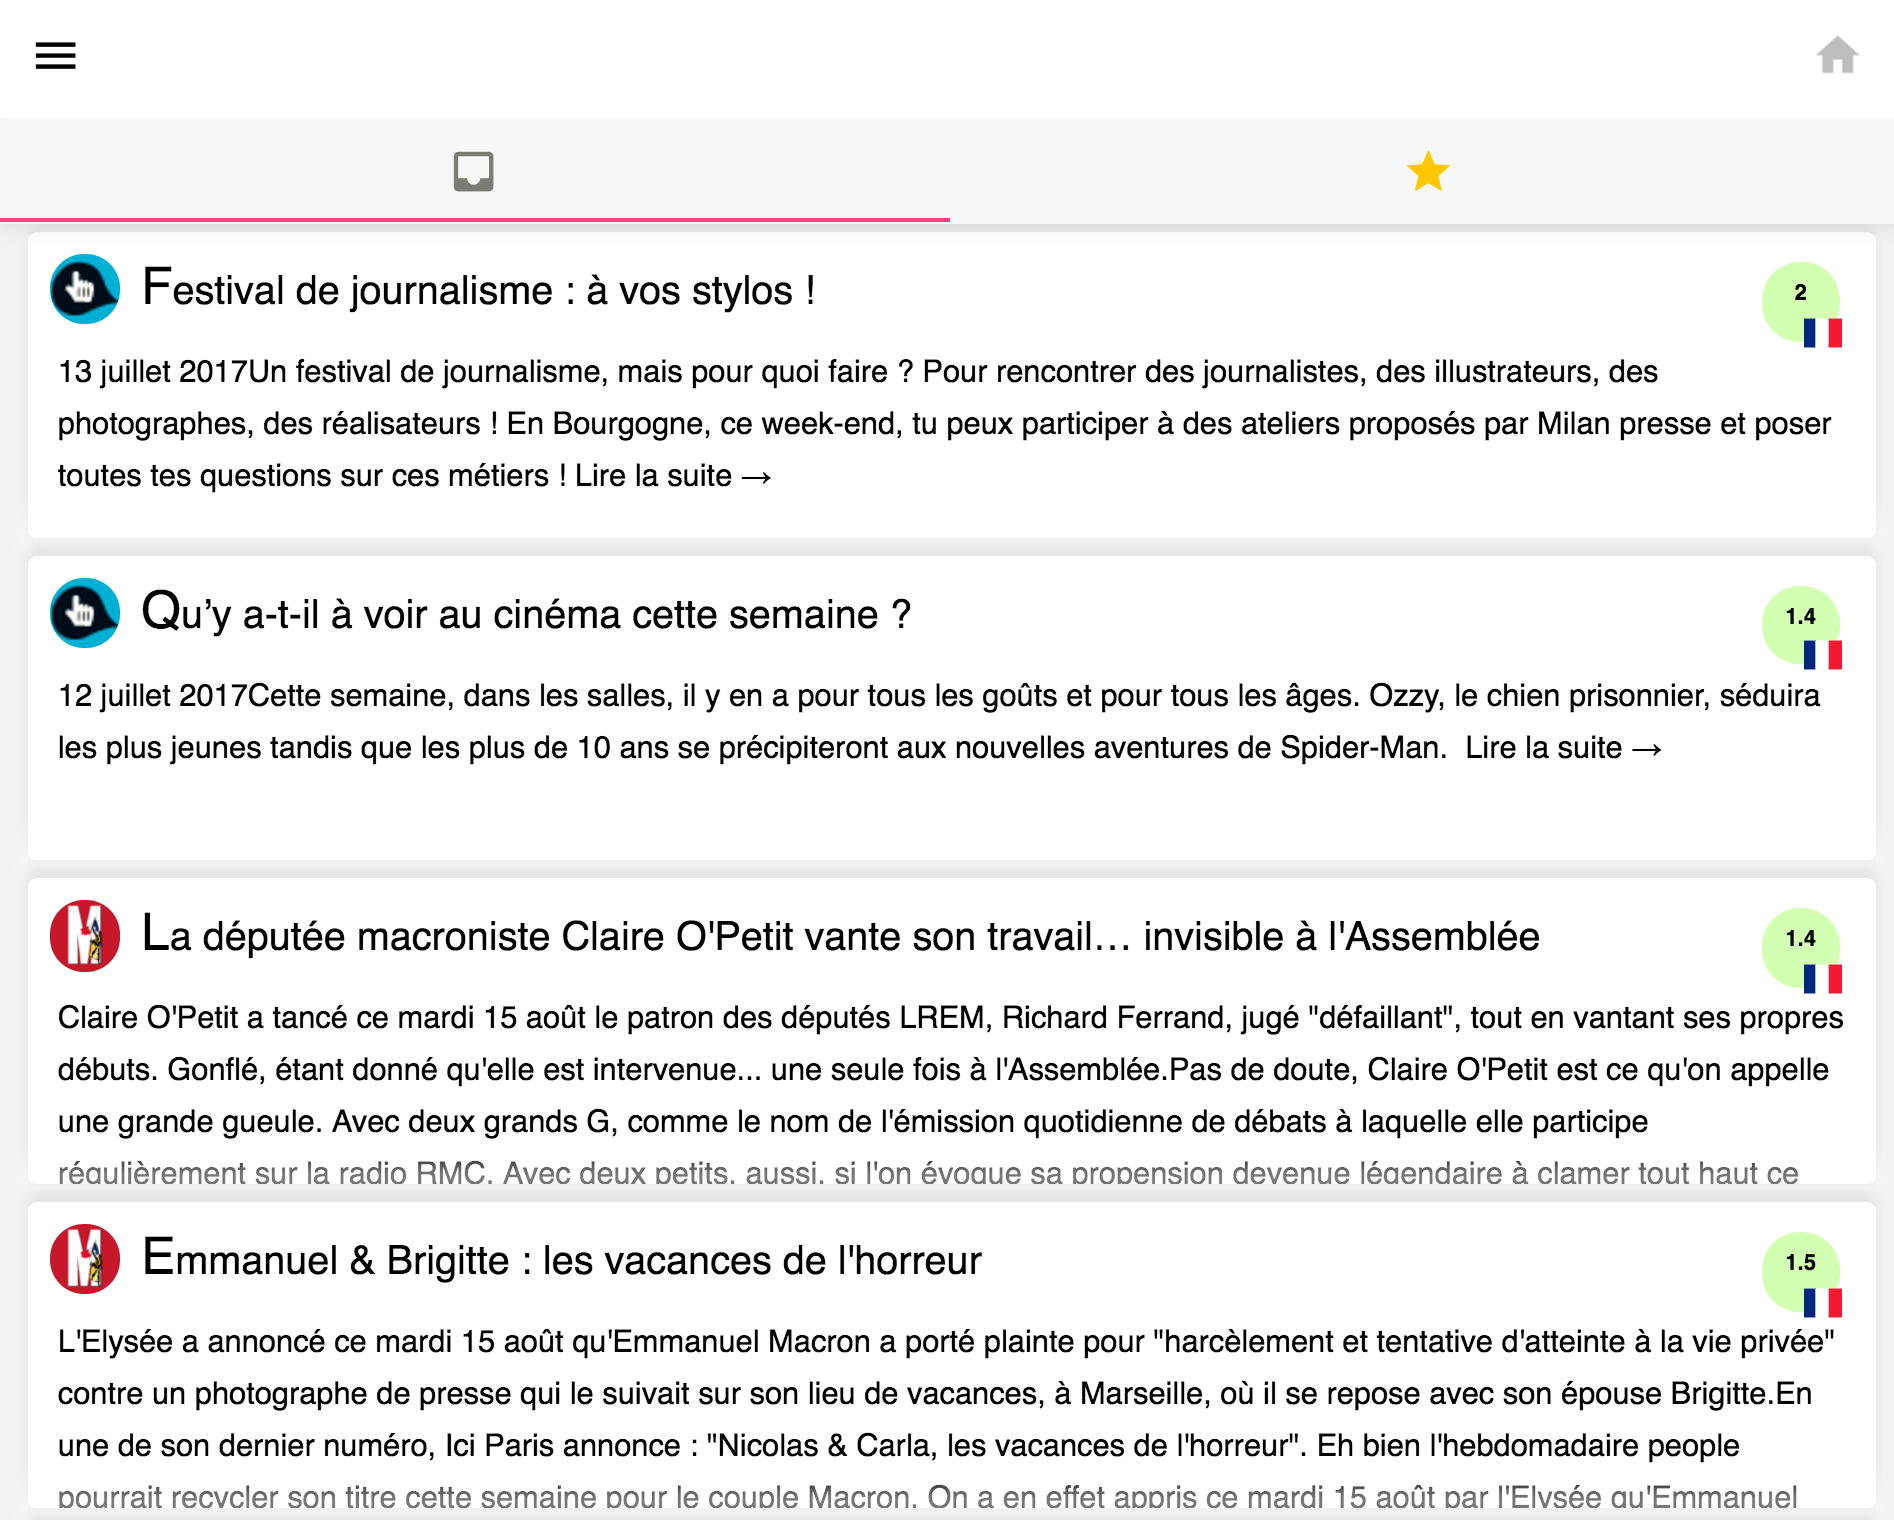
\includegraphics[width=0.95\columnwidth]{figures/article_listing}
      \caption{Article listing presents the source, a summary of the article, and an estimated difficulty level of the article }~
      \label{fig:registrations}
    \end{figure}


In order to properly visualize the reading difficulty of an article in an intuitive manner, there are three levels of information displayed here. First we display a flag representing the language of the article. This is so because a learner could be actually registered to feeds in multiple languages. Second, we allow the user to rapidly judge difficulty on an intuitive level by color coding the difficulty from green to yellow to red. When a particular article has grasped the user's attention, we allow for a more cognitive judgment by scoring the article from 0 to 5 in difficulty.

\ml{TODO: write about how is difficulty estimation done currently}



\subsection{The Text Reader}

The goal of the reader is to make reading as facile as possible. To do this we optimized for the most frequent action that a reader might want to perform: translating a word. 

We explored several types of interactions and we settled on the following: a user clicks on a word, a translation is inserted right after the word, as Figure \ref{fig:translated_word} illustrates: 

\begin{figure}[h!]
\centering
  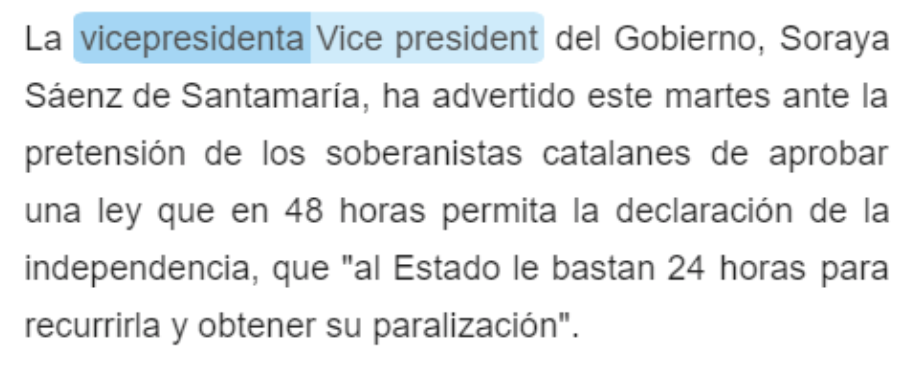
\includegraphics[width=0.8\columnwidth]{figures/translated_word}
  \caption{A translated word is inserted after the tapped word.}~\label{fig:translated_word}
\end{figure}

Ohter alternatives that we explored and eventually dropped for each had disadvantages were: 
\begin{description}

  \item [Temporarily showing a popup of the translation] and then hiding it again. This had the disadvantage of in the case of a more difficult sentence the reader forgetting the word at the begining of the sentence by the time he arrived to the end, and having to re-translate it. 

  \item [Using the native selection mechanism] to select text as opposed to click / touch. We experimented with allowing the learner to select a word in the same way this is normally done on the corresponding platform. This is not a viable solution since native selection is clumsy and slow (e.g. on Android a user must hold their fingertip down for almost a second before the contextual menu is displayed). 
\end{description}


\subsubsection{Chaining Multiple Adjacent Translations}
The user can chain a few consecutive words into a single translation by simply tapping adjacent words which are automatically merged in a translation bubble (Figure \ref{fig:translation_extension}). This is useful for collocations and in cases where by expanding the translated set of words the precision of the translation increases. 

    \begin{figure}[h!]
    \centering
      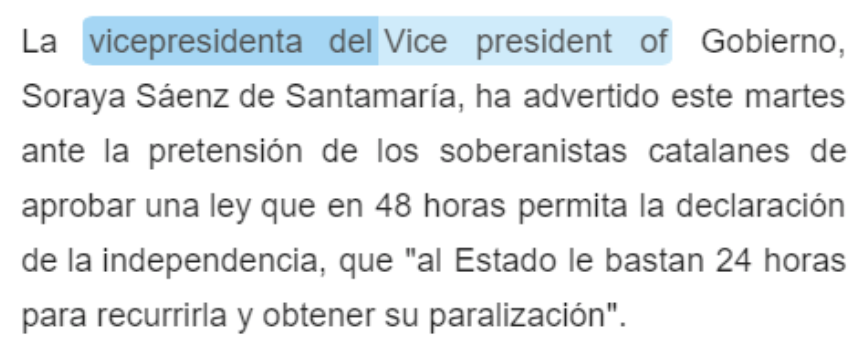
\includegraphics[width=0.8\columnwidth]{figures/translated_words1}
      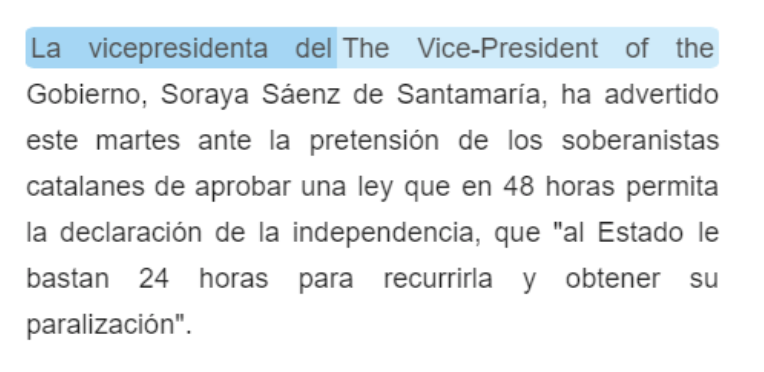
\includegraphics[width=0.8\columnwidth]{figures/translated_words2}
      \caption{When adjacent words are tapped the translation bubble is extended accordingly}~\label{fig:translation_extension}
    \end{figure}

This minimalistic interaction model serves a double purpose - it enables and eases the translation of several chained words but it discourages users from translating entire sentences or phrases. This is good because it is in line with the recommendations of the literature (e.g. Renandya argues that extensive reading should discourage intensive use of translations\cite{renadya07-power}) but also because it reduces the amount of characters which are being translated by the learner (and thus the costs of the system, since some of the translation services have a per-character fee). 

One of the limitations of this interaction is that it is not clear (at least at the moment) how to expand it for the situations in which expressions are present that are composed of words which are not adjacent (e.g. particle verbs in German and Dutch).


\subsubsection{Alternate Translations}
Due to the limitations of machine translation multiple translations might be possible in a given context. In such a case the system will insert the most likely alternative as described earlier right after the selected text, but it will allow the reader to discover alternatives. With a click on the translation, a drop-down menu appears in which alternatives are presented. Figure \ref{fig:registrations} shows that besides the predefined alternatives the learner can provide their own translation via an input box (the third line, ``took place'' is typed in by the learner in the figure). 


\begin{figure}[h!]
\centering
  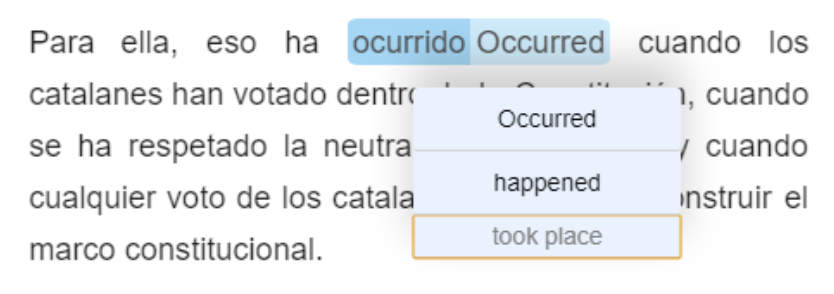
\includegraphics[width=0.8\columnwidth]{figures/translation_alter_menu}
  \caption{A translated word is inserted after the tapped word.}~\label{fig:registrations}
\end{figure}

\subsubsection{Pronounciation}
One of the features that we added following a suggestion of an early beta-tester was the pronounciation of a given word. It has turned out to be a popular feature. Currently the pronounciation of a word or a group of words is the action associated with tapping on the highlighted translated word. The pronounciation is being generated by the default text-to-speech engine of the Chrome browser. \ml{could ask the users if they are happy with it.}

% Although no user has yet complained about it, this means that a user can not pronounce a word without it being translated first. It might also be that for some languages this is more important than for others, and we just did not have users learning those languages (e.g. Danish is notoriously hard to pronounce). In the future we plan to expand the interaction modes to allow pronounciation to exist seperately from translation.

\subsection{The Vocabulary Trainer}

Given the list of words that a user does not know we can generate exercises for them based on their past readings.

Figure \ref{exercise_translate} shows such a generated exercise which asks the reader to translate a given word in the context in which it was encountered in a past reading. The various interactive elements (IEs) that are present in this exercise (and in some of the other exericses are): 

\begin{description}
	\item [A Hint button (IE1)] presents the correct answer.
	\item [Check the answer (IE2)] verifies answer correctness.
	\item [Word pronunciation (IE3)] sounds the pronounciation.
	\item [Control (IE4)] over the exercise card allows for reporting or deleting the exercise.
	\item [Input box (IE5)] allows for entering a solution.
\end{description}

\begin{figure}[h!]
\centering
  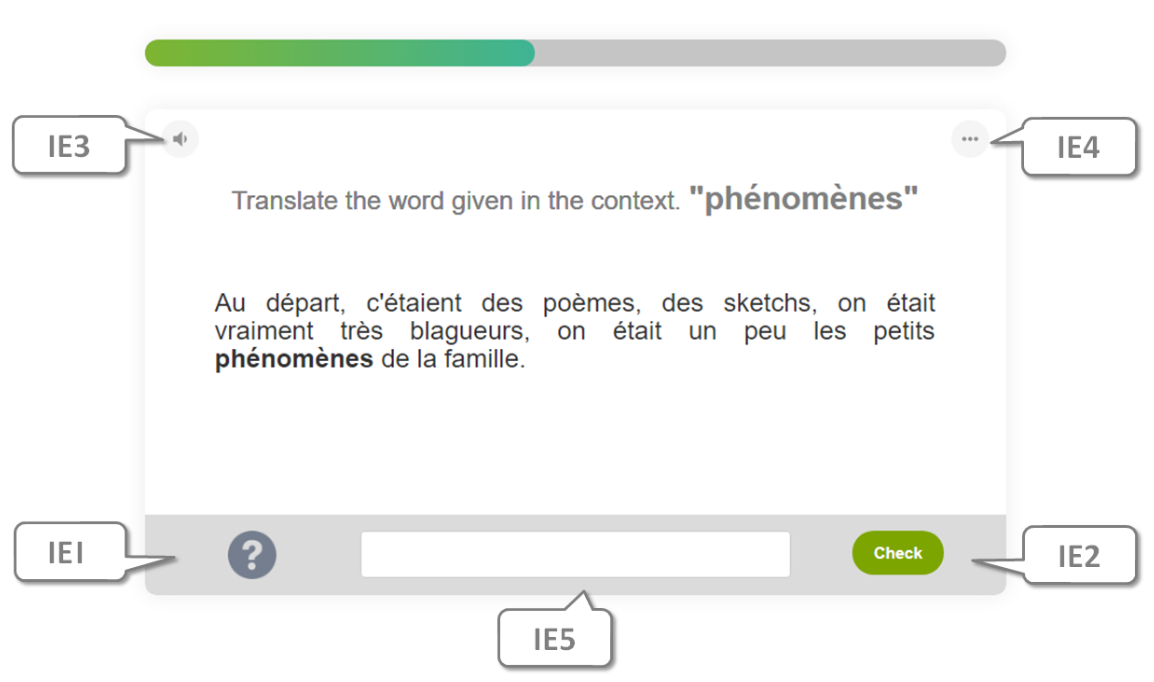
\includegraphics[width=\columnwidth]{figures/exercise_translate}
  \caption{One of the exercise types with which the user is presented asks the user to translate a word in a context that is retrieved from the user's past readings}{
  \label{exercise_translate}
  }
\end{figure}

\subsubsection{Prioritizing Words to Study}

Since a learner might encounter many words that are not understood, we need to prioritize those that are to be studied in exercises. We use three aspects to prioritize words: 

% The words good for study are the ones that are either starred by the user, or are important and of quality based on a set of heuristics. 

\begin{description}

  \item [Important Words] are the ones which appear frequently in the language. For word frequencies we use frequencies computed based on movie subtitles which have been shown to be highly representative to frequencies in human interacitons \cite{New07-subtitles}. 
  
  \item [Quality Context] we favor words that come with a context which is not too short but not too long. 

\end{description}

\subsubsection{Scheduling Exercises}

The scheduling algorithm is based on an adaptive, response-time-based scheduling algorithm [was developed] to increase the efficiency of perceptual learning by Mettler et al. \cite{Mettler14-ARTS}. After evaluating several alternative scheduling strategies we settled on the Mettler one since it has been proven to have gains with both familiar, seen items as well as with new, unseen instances and the benefits of adaptive scheduling were present at an immediate test as well as at a delay \cite{Mettler14-ARTS}.



One of the problems with this is that sometimes the context is too long and sometimes 


\subsection{Translation Service}

The translations are provided by our server. The main advantage of this indirection is that this allows the server to track the words that are looked up and the context (sentence) in which they are being looked up. This information is then used for estimating learner knowledge and for generating later personalied exercises. 

To avoid depending on a single service and to also increase the likelihood that at least one of the alternative translations is the correct one, the translation service dispatches in parallel requests to at least three third party translation APIs: Google Translate, Microsoft Translate, and Glosbe -- a free translation API. The first two provide contextual translations and multi-word translations, while the third is a simple dictionary. 

The dependency of the translation service on multiple third party APIs allows for a higher reliability and a chance to guarantee a low response time: when a service is down or too slow to respond, the results from it are ignored.

\subsection{The Teacher Dashboard}

Although not the focus of this paper, since the system does not need to be used in a formal classroom, the system has also a dashboard for the teacher. The teacher can see the history of what his students have read and observe their chosen translations in context.






